\documentclass{hfutpaper}
\usepackage[urlcolor=blue]{hyperref}
\usepackage{threeparttable}
\usepackage{setspace}
\usepackage{titlesec}
\usepackage{float}
\newcommand{\upcite}[1]{\textsuperscript{\textsuperscript{\cite{#1}}}}
\usepackage{fancyhdr}
\titleformat{\section}{\large \heiti}{\chinese{section}、}{0em}{}
\begin{document}
\begin{center}
\LARGE
  \textbf{信息传输}\\
  \vspace{0.2em}
  \large
    作者:R. V. L. Hartley \\
    
  {\small 译者:李晓峰}\footnote{来自于网络空间安全经典论文翻译项目\url{https://gitee.com/uisu/InfSecClaT}}\\
  {\small (北京联合大学智慧城市学院,cy\_lxf@163.com)}\\
  
  \end{center}
\rule[0.1\baselineskip]{\textwidth}{0.5pt}
\textbf{梗 \ 概}\\
\large
本文提出了基于物理的而非心理上的信息的量化度量。本文从瞬态的角度讨论了能量存储引起的失真如何限制信息在系统上的传输速率。回顾了瞬态和稳态视角之间的关系。结果表明,当能量存储用于将稳态传输限制在有限的频率范围内时,可传输的信息量与可用时间频率范围宽度的乘积成正比。文中列举了几个实例,说明了这一原理在实际系统中的应用。在图像传输和电视的情况下,强度的空间变化通过稳态方法进行分析,类似于通常用于随时间变化的方法。
\\
\rule[0.1\baselineskip]{\textwidth}{0.5pt}


\section{信息的度量}

\subsection{心理因素的消除}

\subsection{(完成翻译)信息的量化表示}
每一次选择,可以选三个可能的符号(symbol),两个连续选择共有$3^2$或9中符号序列的可能性,n个选择就是$3^n$种可能。假设不是使用三个电流值的系统,而是提供一个系统,其中任意数量的不同电流值可传输于线路,并在接收端进行区分。
对于这个系统来说,每次可以的选择是s个,可区分的序列是$s^n$。
\par

对于Baodot型的电传打字系统,操作员选择字母或其它字符,每个字符由一系列符号组成(通常是五个符号)。我们可以将各种不同电流值视为基本符号,将不同符号序列代表的字符看作二级符号(secondary symbols)。发送端在基本或者二级符号中进行选择,假设操作员选择了$n_2$个字符的序列,每个字符由$n_1$个基本符号组成,在每次选择时,他将获得不同的二级符号,每个二级符号是其在基本符号中进行了$n_1$次选择形成的不同序列。如果我们将二级符号的数量记为$s_2$,那么
\[s_2=s^{n_1} \qquad \qquad (1)\]
对于Baudot系统
\[s_2=2^5=32 \text{字符} \qquad \qquad (2)\]
我们可以从二级选择数$n_2$推出可能二级符号序列满足
\[s_2^{n_2} = s^{n_1 n_2} \qquad \qquad (3) \]
现在$n_1 n_2$是基本符号的选择数n,如果没有将基本符号分组为二级符号的机制,则生成相同序列所需的基本符号选择数就是n。因此,我们看到,无论是否出于解释目的对基本符号进行分组,可能序列的总数都是$s^n$。


$s^n$是可能序列数,我们希望它可以用于度量信息。让我们看看他是如何满足度量需求的。


对于特定系统和操作模式,可以假设s是固定的,并且选择数n随着通信进行而增加。因此,在这种理解中,传输的信息量将随着选择的数量呈指数增长,单个选择对传输的总信息的贡献将逐渐增加。毫无疑问,从心理学的角度来看,这种增长确实经常发生在交流中。例如,在一场旷日持久的讨论结束时,一个词“是”或“否”可能具有非常重要的意义。然而,这种情况是例外,而不是“规则”\footnote{译者注:这里原文是rule,作者应该想表达的是,“这不是规律”}。讨论主题的不断变化,甚至涉及到的参与人的不断变化,使得在实践中都会由这样的结果,就是会将这种指数关系的累积作用限制在相对较短的时间内。


此外,我们正在制定一项独立于心理因素的度量。当我们考虑物理传输系统时,我们发现在设备中传输连续选择结果时,没有这样的指数增加。所涉及的各种基本符号,在接收端一个基本符号选择与另一个基本符号选择都是一样可区分。电报系统发现一条十个字符电报并不比一个字符电报更难传输。现在成功传输语音的电话系统将继续这样做,只要该系统保持不变。为了使信息测量具有实际工程价值,应该满足:信息应与选择的数量成比例。因此,可能序列的数量不适合直接用作信息的度量。


然而,我们可以将其用作度量的基础,衍生出满足实际要求的度量方法。为了做到这一点,首先信息量与选择数成比例,因此选择比例因子,使等量的信息对应于等量的可能序列。对于一个特定的系统,信息量与n个选择相关的关系为
\[H=Kn \qquad \qquad \qquad (4)\]
此处K是常量,依赖于每次选择时符号s的数量。取s的值为$s_1$和$s_2$的任意两个系统,相应的常数为$K_1$和$K_2$。然后,我们通过以下条件定义此常数:当两个系统的选择数$n_1$和$n_2$使得两个系统的可能序列数相同时,两个系统的信息量也相同;也就是说,当
\[s_1^{n_1}=s_2^{n_2}\qquad \qquad \qquad (5)\]
\[H=K_1n_1=K_2 n_2 \qquad \qquad \qquad (6)\]
我们可得\footnote{
	译者注:对于(5),等式两边同时取log,有$n_1\log{s_1} = n_2 \log{s_2}$,进一步有$\frac{n_1}{n_2} =\frac{\log{s_2}}{\log{s_1}}$,对于等式(6),有$\frac{n_1}{n_2} =\frac{K_2}{K_1}$,结合上面推导有$\frac{K_2}{K_1}=\frac{\log{s_2}}{\log{s_1}}$,即$\frac{K_2}{\log{s_2}}=\frac{K_1}{\log{s_1}}$
}
\[\frac{K_1}{\log{s_1}} = \frac{K_2}{\log{s_2}}  \qquad \qquad \qquad (7)  \]
这个关系对于所有s的取值都成立,只要K与s的关系如下所示
\[K=K_0 \log{s} \qquad \qquad \qquad (8) \]
此处$K_0$对所有的系统都一样。我们可以取任意的数为对数的底,因此$K_0$也是是任意的,所以我们可以忽略掉$K_0$。选择一个特定的对数底确定了信息的度量单元。将K的值带入(4)中\footnote{译者注:此处是将(8)中的K值带入(4)}
\[H=n\log{s} \qquad \qquad \qquad (9)  \]
\[H= \log{s^n} \qquad \qquad \qquad (10) \]
我们所做的就是把可能的符号序列数的对数作为信息的实际度量。


这种情况类似于在电话系统中加入一个设备测量传输损耗的情况,加入设备的效果是以一定比例改变传递给接收器的功率,这个比率可以用来衡量损失,人们发现用功率比的对数来衡量传输损耗更方便。


如果我们把n看成单位(unity),我们会看到与单个选择相关的信息是可用符号数的对数表示;例如,在上面提到的Baudot系统中,主符号或电流值的数量是2,一个选择的信息量是$\log{2}$;一个字符包含5个选择的信息量是$5\log{2}$。如果我们将一个字符视为二级符号,并取这些符号数量的对数,即$\log{2^5}$或$5\log{2}$,则会得到相同的结果。与100个字符相关的信息将是$500\log{2}$。信息的数值取决于使用的对数系统,将当前值的数量从2增加到10,即比率5,信息量增加比值为$\frac{\log{10}}{\log{2}}$,即3.3。它对传输速率的影响将取决于选择的速率如何受到影响\footnote{译者注:这里的“选择的速率”是指信源的变换速度}。这将在稍后讨论。


如刚才所考虑的情况,当二级符号都涉及相同数量的基本选择时,关系非常简单。当使用非统一代码的电报系统时,情况就相当复杂。一个比实际困难得多的困难来自这样一个事实,即给定数量的二级或字符选择可能需要大量不同数量的基本选择,这取决于选择的特定字符。这似乎表明,从基本符号和二级符号推导出的信息量是不同的。然而,可以很容易地证明,这并不会发生。如果发送者在任何时候都可以自由选择任何二级符号,他可以在包含最多基本符号中进行所有选择。然后,二级符号都将具有相同的长度,并且,与统一编码一样,基本符号的数量将是字符数与最大二级字符数的乘积。如果给定数量字符的基本选择数量要保持在比这个更小的值,则必须对二级符号的选择自由施加一些限制。如果在发送信息时不超过每个字符分配的点数,一般来说,操作员必须避免选择比其平均出现率更长的字符。在本讨论的语言中,我们可以说,对于某些$n_2$二级选择$s_2$的值,也就是二次符号的数量,减少到,所有字符的信息量的和等于所涉及的基本选择总数所推到出来的信息量。这可以写为
\[\sum_{1}^{n_2}\log{s_2} =n \log{s} \qquad \qquad  \qquad (11)\]
此处n是基本符号的数量或与$n_2$个字符关联的点的长度,这表明,基本符号为度量信息提供了基础。



迄今为止的讨论主要涉及电报。当我们试图将这一观点推广到其他形式的交流时,需要做出某些概括。例如,在语音中,我们可以假设基本选择代表连续单词的选择。在此基础上,s将代表可获取的单词数,对于对话的第一个单词,这将对应于语言中的单词数。对于后续选择,数值通常会减少,因为后续单词将以可理解的方式与之前的单词组合。然而,这种限制只是解释的限制,系统同样能够传输一种语言中所有可能的单词排列都可以理解的通信\footnote{译者注:这就是说虽然由于语言的约定,前后会有限制,但是从系统角度说,他仍然时可以传输所有情况的。}。
此外,电话系统也同样能够用一种语言\footnote{译者注:这里的另一种语言,指的时另一种编码方式。}传输语音。每一个词都可以用各种各样的方式说,也可以用更丰富的方式唱。与单个口语单词的选择相关的大量信息表明,该单词最好被视为二级符号或基本符号序列。让我们看看这个观点会把我们引向何方。
\par

\begin{figure}[htp]%H表示图强制在下面,想设置浮动环境用htp
	\centering  %插入的图片居中表示
	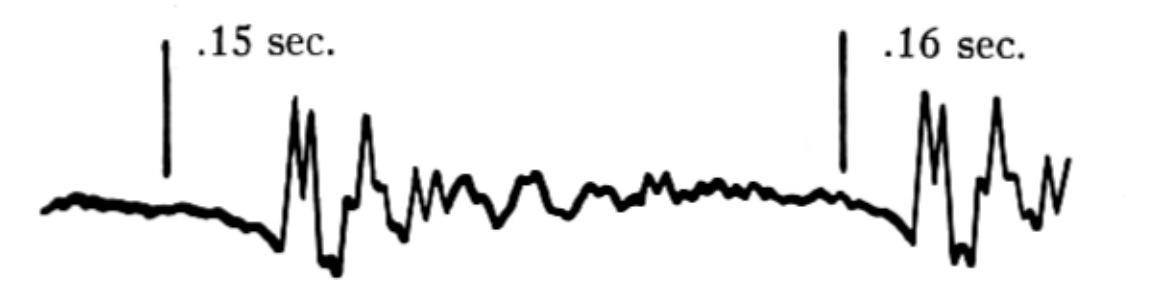
\includegraphics[scale=0.5]{magnitude-time.png}  %插入的图,包括JPG,PNG,PDF,EPS等,放在源文件目录下
	\caption{语音波形}  %图片的名称
	\label{fig2}
\end{figure}

单词的实际物理表达是一个声学或电扰动,其可表示为图\ref{fig2}的幅度-时间函数,是语音的波形记录。这个函数在其他通信模式中也很典型,稍后将详细讨论。然后,我们必须检查这种连续函数传递信息的能力。显然,在任何给定的时间间隔内,幅度可能会随着无限多个这样的函数而变化。这意味着可能的二级符号数量将是无限的,因此信息量也将是无限的。然而,在实践中,所包含的信息是有限的,因为发送方无法完全准确地控制函数的形式,而函数形式的任何扭曲都会导致它与其他函数混淆。\par

\begin{figure}[htp]%H表示图强制在下面,想设置浮动环境用htp
	\centering  %插入的图片居中表示
	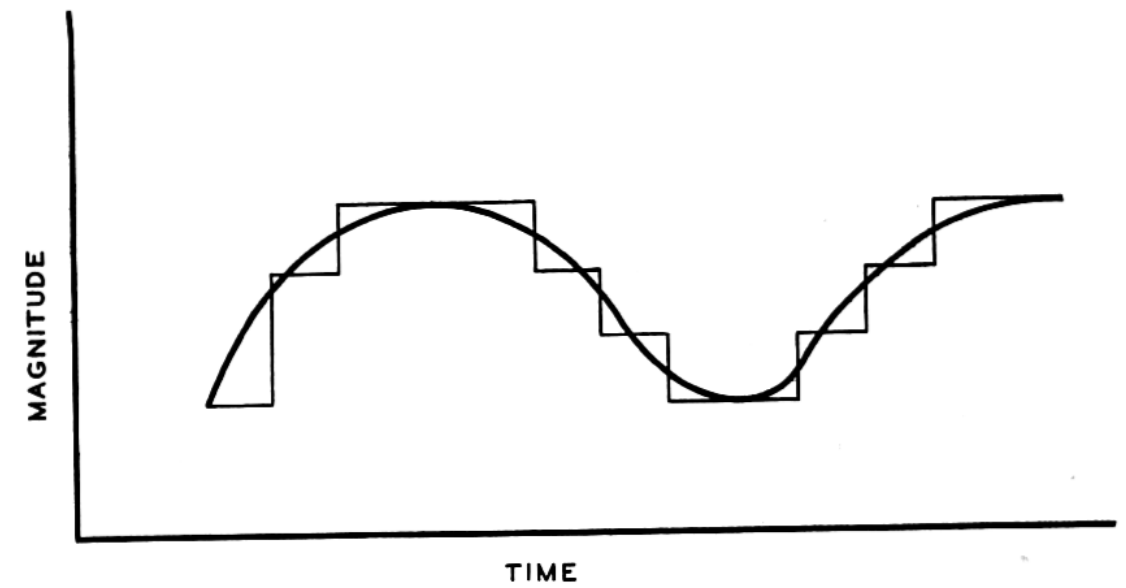
\includegraphics[scale=0.5]{magnitude-time-digital.png}  %插入的图,包括JPG,PNG,PDF,EPS等,放在源文件目录下
	\caption{阶梯语音波形}  %图片的名称
	\label{fig3}
\end{figure}

连续曲线可以被认为是由连续阶梯组成的曲线近似,如图\ref{fig3}所示,当两阶梯之间的间隔被设置为无穷小时,可以无限趋近连续曲线。一条定义不完善的曲线可以被认为是两个阶梯之间的间隔是有限的。这些阶梯代表基本选择。在有限时间内,基本选择数量是有限的。此外,在每一个台阶所做的改变被认为是有限数量的值中的一个。这意味着可用符号的数量是有限的。如果情况并非如此,则曲线将在每一阶梯完全精确地定义,这意味着在任何一步进行的观察将提供无限多个可能的值。下图\footnote{译者注:此处的下图,就是图\ref{fig3}}显示离散选择和相应连续曲线之间的关系。我们可能会想到一辆装有特殊类型转向装置的自行车,这种装置允许骑手将前轮设置在有限的固定位置。在这样一台机器上,他试图以这样一种方式骑行,即前轮沿着一条不规则的曲线行驶,他完成的精度将取决于转向机构之间的距离,以及他能够设置的位置的数量。\par

通过这种或多或少的人工装置,电话中使用的连续幅度-时间函数,受到与电报中相同类型的连续离散处理。\par

\section{通信速率}

\subsection{符号间干扰的限制}

\subsection{与阻尼常数的关系}

\subsection{与能量储存的关系}

\section{稳态和瞬态视角}

\section{频率范围与时间乘积的意义}

\subsection{将消息与行匹配}

\subsection{在图像传输中的应用}

\subsection{在电视中的应用}

\section{结论}

\end{document} 